\subsection{Implementation}
We implement a framework in order  to simplify parameter estimation for 
pulse-chase RNA-seq experiments. 
We use \emph{R} programming environment, 
because it allows very flexible handling of user-specified models, 
includes implementations a variety of commonly used procedures and 
has powerfull plotting features \citep{rlang}.
\par A user needs to provide
\begin{itemize}
 \item a count table with the raw read numbers
 \item a condition matrix (to infer sample fractions in the count table)
 \item formulas for the mean read numbers, e.g. 
 $r_\text{L}\sim \mu e^{-dt}$, (section~\ref{subsec:kinetics}).
 \item spike-ins, if relevant
\end{itemize}
The package utilizes so-called \emph{computing on the language},
a feature of the \emph{R} language \citep{team2000r}.
This allows to handle arbitrary formulas, which the user supplies for 
the mean gene expression levels. Hence, no manual 
implementation for the likelihood functions is necessary and the 
formulas are needed to defined only once.
\subsection{Evaluation using simulated data}
To demonstrate the analysis workflow, we generated a data 
set on the basis of the pulse-model, introduced in the section~2.
\begin{align}
 r_\text{i,T}&=\mu_i\\
 r_\text{i,L}&=\mu_i \left(1-e^{-d_it_\text{L}}\right)\\
 r_\text{i,U}&=\mu_i e^{-d_it_\text{L}},
\end{align}
where $t_\text{L} = 12$ hr is the time amount of pulse-labelling,
$i \in 1..100$ is a gene index, $\mu_i$ and $d_i$ are gene-specific parameters,
which are sampled from random number generator.
Usually concentration of RNA in the samples is normalised before the
sequencing procedure \citep{}. This introduces a bias, which 
we model by fraction coefficients in section~\ref{subsec:normalisation}. 
For this data set,  the fraction-specific normalisation factors are 
$n_\text{total}$=1 ({reference fraction}),
$n_\text{label}$=2,
$n_\text{unlab}$=3.
\par 
On the basis of this parameters,  we sampled read counts from the NB distribution 
with the dispersion parameter $\alpha=0.01$,  in 3 replicates for 
every fraction ($(\text{total, label, unlab})\times(\text{replicates 1,2,3})$).
Using this simulated count data,  we evaluated the performance of the developed
\verb|pulseR| package.
\par
To improve the fitting procedure, we provided the initial guess for the expression level
on the basis of the median read count in the total fraction.
The initial values for the degradation rates were chosen as random numbers.
The predictions for every gene in three different fractions demonstrate
good quality of fitting, fig.~\ref{fig:predictions}. The relative errors of
the parameter fits is worse for the lower expressed genes, fig.~\ref{fig:errors}.
That is expected to occur, because the dispersion of the NB-distributed values
is higher for the data with a lower mean.
\begin{figure}
 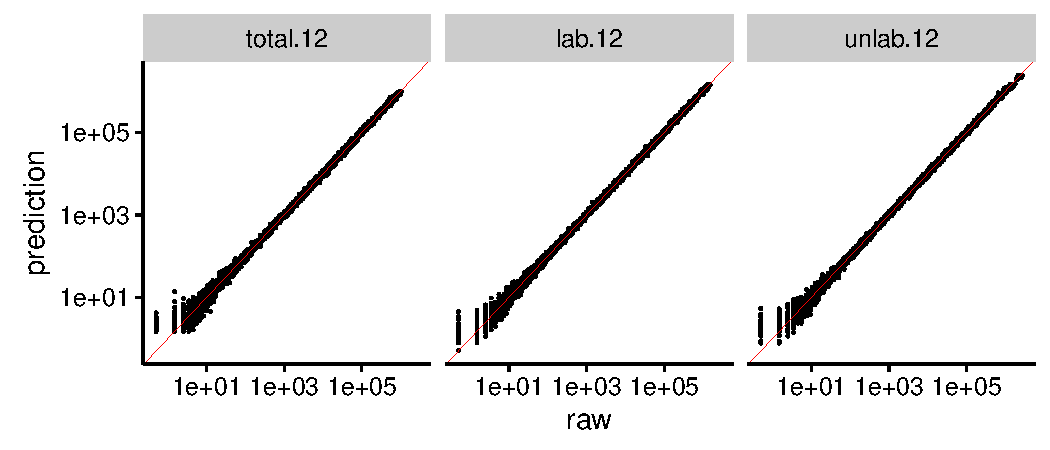
\includegraphics[width=\linewidth]{fig/predictions}
 \caption{Comparison of the model \emph{predictions} to the generated 
 \emph{raw counts} for 3 different fractions (total, labelled, unlabelled)
 at after 12 hr of pulse-experiment.}
 \label{fig:predictions}
\end{figure}

\begin{figure}
 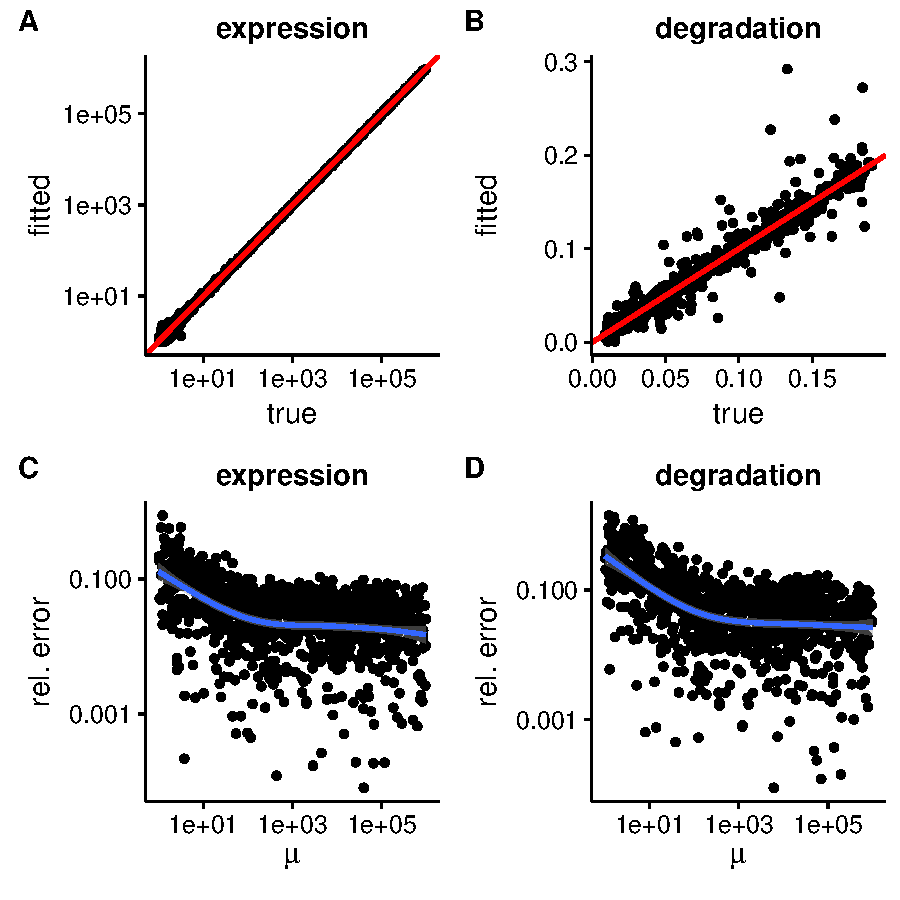
\includegraphics[width=\linewidth]{fig/parameters}\\
 \caption{Comparison of the fitted and true parameter values (A, B) and 
 relative errors in the parameter fit (C, D) for the expression level $\mu$ 
 and the degradation rate $d$.}
 \label{fig:errors}
\end{figure}